\documentclass[10pt,a4paper]{article}
\usepackage{fontspec}
\usepackage{amsmath}
\usepackage{amsfonts}
\usepackage{amssymb}
\usepackage{graphicx}
\usepackage[left=1.00in, right=1.00in, top=1.00in, bottom=1.00in]{geometry}
\usepackage[colorlinks=true,
			linkcolor=blue]{hyperref}
\usepackage{cleveref}
\usepackage{minted}
\usepackage{lmodern}

\begin{document}
	\title{Assignment 1}
	\author{Daniel Celis Garza}
	\date{\today}
	\maketitle
	
	Using the Debye length, $\lambda_{D}$ and the ion speed of sound $c_{s}$,
	\begin{align} \label{eq:constants}
		\lambda_{D} = \sqrt{\dfrac{\epsilon_{0} T_{e}}{e n_s}} \qquad
		c_{s} = \sqrt{\dfrac{e T_{e}}{m_{i}}},
	\end{align}
	we normalise the relevant quantities to
	\begin{align} \label{eq:norm}
		\hat{x} = \dfrac{x}{\lambda_{D}} \qquad
		\widehat{n_{i}} = \dfrac{n_{i}}{n_{s}} \qquad
		\widehat{n_{e}} = \dfrac{n_{e}}{n_{s}} \qquad
		\hat{\phi} = \dfrac{\phi}{T_{e}} \qquad
		\hat{E} = \dfrac{\lambda_{D}}{T_{e}} E \qquad
		\widehat{v_{i}} = \dfrac{v_{i}}{c_{s}} \qquad
		\widehat{v_{s}} = \dfrac{v_{s}}{c_{s}}.
	\end{align}
	Taking the equations for electron density, ion continuity and energy conservation respectively,	
	\begin{subequations}
		\begin{align} \label{eq:edicec}
			n_{e}(x) &= n_{s} \exp\left(\dfrac{\phi(x)}{T_{e}}\right)\\
			n_{i}(x) v_{i}(x) &= n_{s} v_{s} \\
			\frac{1}{2} m_{i} v_{i}^{2}(x) &= \frac{1}{2}m_{i} v_{s}^{2} - e \phi(x),
		\end{align}
	\end{subequations}
	Ignoring the dependence on $\hat{x}$ for clarity and substituting the normalised values from \cref{eq:norm} into \cref{eq:edicec} and recalling the value for $c_{s}$ from \cref{eq:constants}, we obtain expressions for $\widehat{n_{e}},~\widehat{n_{i}} \textrm{ and } \widehat{v_{i}}$ (numbered),
	\begin{subequations}
		\begin{align} \label{eq:nedicec}
			n_{s} \widehat{n_{e}} &= n_{s} \exp\left(\hat{\phi}\right) \nonumber\\
			\widehat{n_{e}} &= \exp\left(\hat{\phi}\right)~, \\
			n_{s} \widehat{n_{i}} c_{s} \widehat{v_{i}} &= n_{s} c_{s} \widehat{v_{s}} \nonumber\\
			\widehat{n_{i}} &= \dfrac{\widehat{v_{s}}}{\widehat{v_{i}}}~, \\
			\frac{1}{2} m_{i} c_{s}^{2} \widehat{v_{i}}^{2} &= \frac{1}{2} m_{i} c_{s}^{2} \widehat{v_{s}}^{2} - e T_{e} \hat{\phi} \nonumber\\
			\frac{1}{2} m_{i} \dfrac{e T_{e}}{m_{i}} \widehat{v_{i}}^{2} &= \frac{1}{2} m_{i} \dfrac{e T_{e}}{m_{i}} \widehat{v_{s}}^{2} - e T_{e} \hat{\phi} \nonumber\\
			\widehat{v_{i}} &= \sqrt{\widehat{v_{s}}^{2} - 2 \hat{\phi}}~.
		\end{align}
	\end{subequations}
	The current,
	\begin{align} \label{eq:current}
		J = e n_{s} c_{s} \left[ \sqrt{\dfrac{m_{i}}{2 \pi m_{e}}} \exp\left(\dfrac{\phi}{T_{e}}\right) - 1 \right]~,
	\end{align}
	can be normalised by substituting the expression for $\hat{\phi}$ from \cref{eq:norm} and dividing by $e n_{s} c_{s}$ to yield the normalised current
	\begin{align} \label{eq:ncurrent}
		\hat{J} = \dfrac{J}{e n_{s} c_{s}} = \left[ \sqrt{\dfrac{m_{i}}{2 \pi m_{e}}} \exp\left(\hat{\phi}\right) - 1 \right]~.
	\end{align}
	\Cref{fig:results} shows the results of numerically solving the normalised equations (numbered and boxed),
	\begin{subequations}
		\begin{align} \label{eq:derivs}
			\dfrac{\mathrm{d}\hat{\phi}}{\mathrm{d}\hat{x}} &= -\hat{E} \\
			-\dfrac{\mathrm{d}^{2}\hat{\phi}}{\mathrm{d} \hat{x}^{2}} &= \dfrac{\mathrm{d} \hat{E}}{\mathrm{d} \hat{x}} = \widehat{n_{i}} - \widehat{n_{e}} \nonumber\\
			-\dfrac{\mathrm{d}^{2}\hat{\phi}}{\mathrm{d} \hat{x}^{2}} &= \dfrac{\mathrm{d} \hat{E}}{\mathrm{d} \hat{x}} = \dfrac{\widehat{v_{s}}}{\widehat{v_{i}}} - \exp\left(\hat{\phi}\right)
		\end{align}
	\end{subequations}
	with $0 \leq \hat{x} \leq 40,~\hat{\phi} = 0,~\hat{E} = 0.001,~\hat{v}_{s} = 1$ using 100 points as well as plotting $\hat{J}$ assuming $\dfrac{m_{i}}{m{e}} \approx 1840$.
	\begin{figure}
		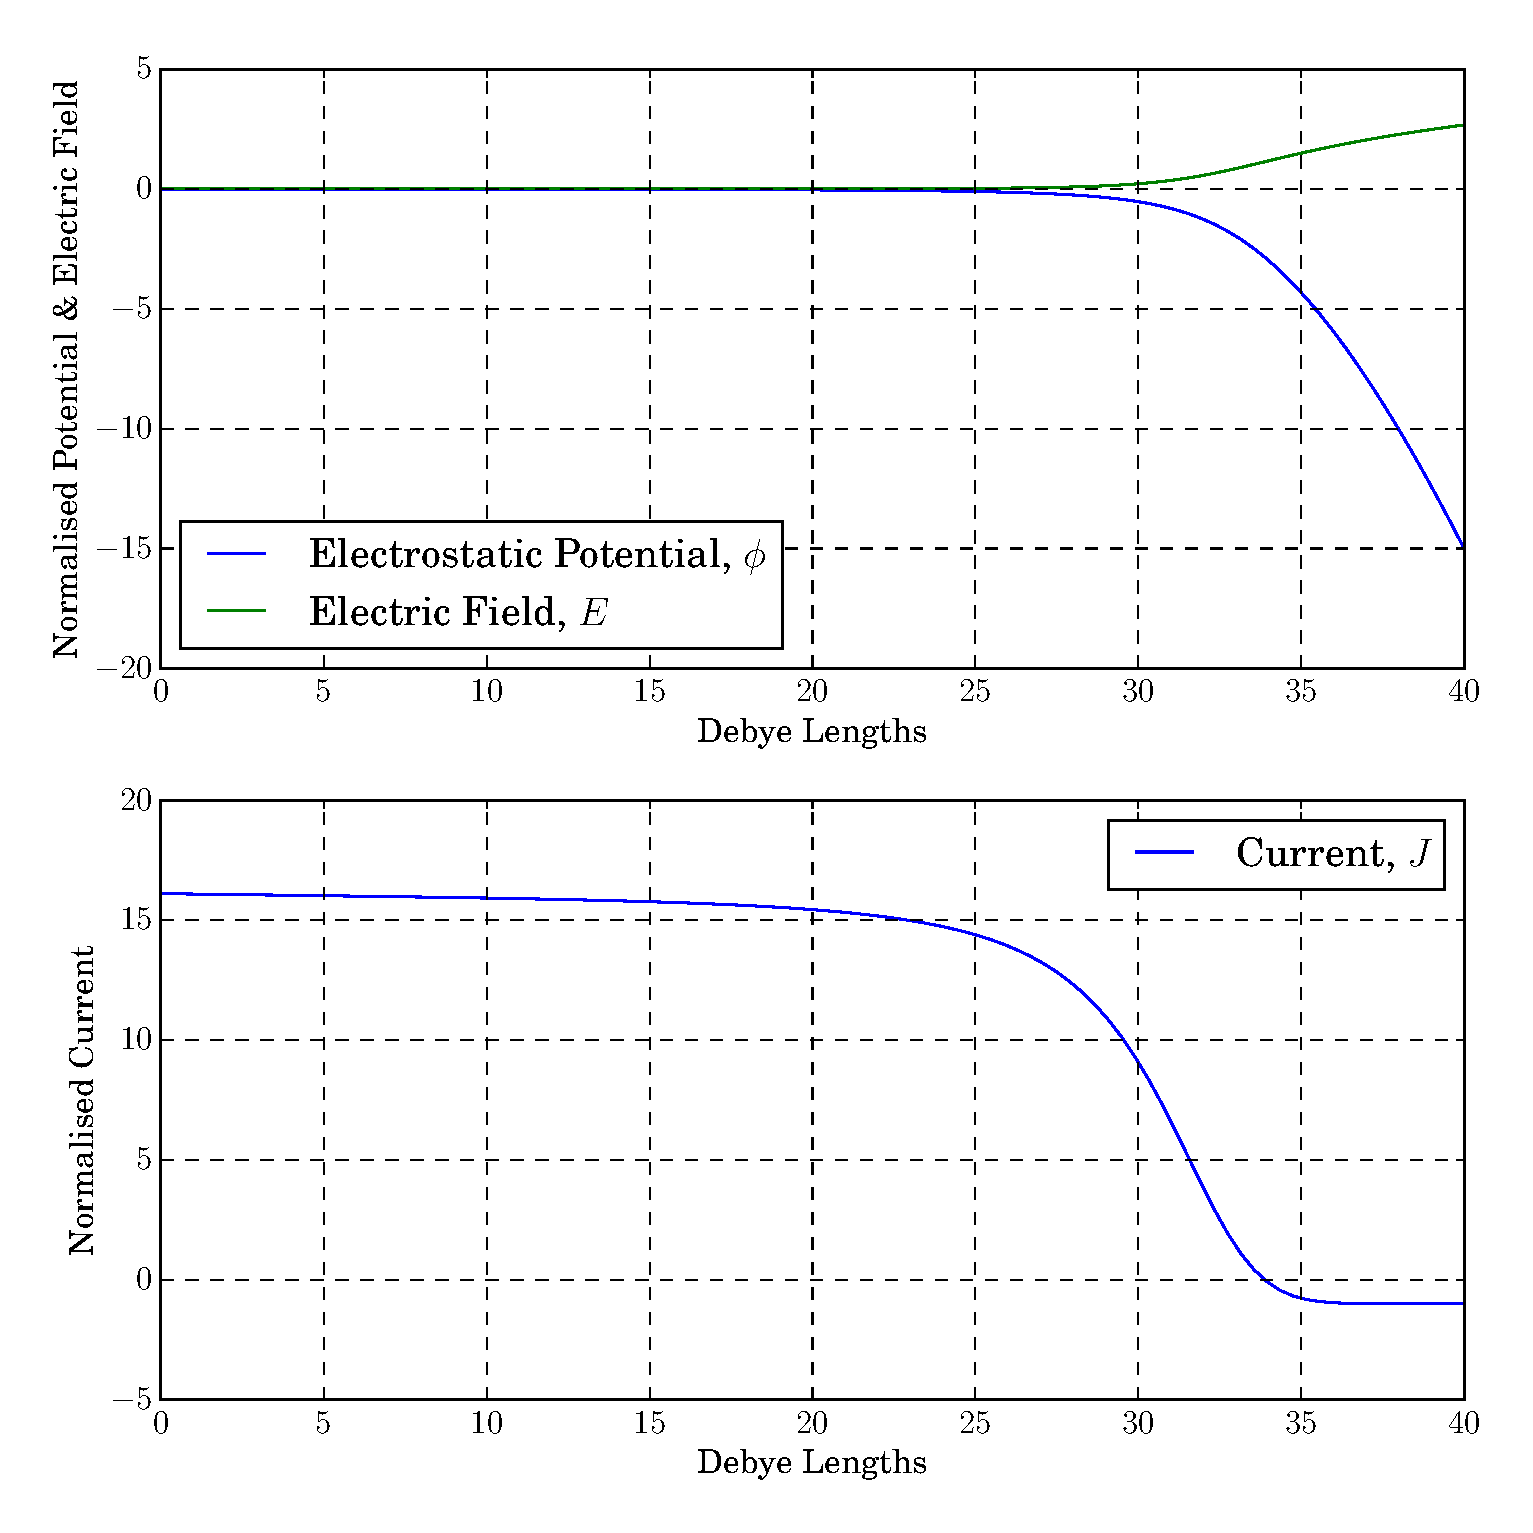
\includegraphics[width=\textwidth]{debye.eps}
		\caption{Results.}\label{fig:results}
	\end{figure}
	The source code is included.
	\inputminted[linenos = true,
				 breaklines, 
				 breakanywhere]{python}{assignment1.py}
\end{document}